%!TEX root = Funktionalanalysis - Vorlesung.tex

\section{Approximation von $L^{p}$ Funktionen}



Sei $x = (x_{1}, x_{2}, \dotsc) \in \ell^{p}, x_{m} = (x_{1}, \dotsc, x_{m}, \dotsc)$. \\
\[ \text{Dann }\|  x - x_{m} \| \rightarrow 0 \text{ für } m \rightarrow \infty. \]
	\newline
Betrachten wir $L^{p}(\Omega)$, mit z.B. $\Omega = \MdR^{d}$ und die Integraloperatoren $T \colon L^{p}(\Omega) \rightarrow L^{p}(\Omega)$
	\[ T f(u) = \int k(u, v) f(v) dv \quad (*) \label{eq:8.0-BeschrOperatorInLp} \]
wobei $k \colon \Omega \times \Omega \rightarrow \MdK$ messbar.

\begin{satz} \label{satz:8.1}
	Sei $k \colon \Omega \times \Omega \rightarrow \MdK$ messbar	und
	\begin{align*}
		\sup_{u \in \Omega} & \int_{\Omega} |k(u, v)| dv \leq C_{1} < \infty \text{ und} \\
		\sup_{v \in \Omega} & \int_{\Omega} |k(u, v)| du \leq C_{2} < \infty
	\end{align*}
	Dann wird durch \hyperref[eq:8.0-BeschrOperatorInLp]{$(*)$} ein beschränkter Operator $T \colon L^{p}(\Omega) \rightarrow L^{p}(\Omega)$ mit
	\[ \| T \|_{L^{p} \rightarrow L^{p}} \leq C_{1}^{\frac{1}{p'}} C_{1}^{\frac{1}{p}}, \quad \frac{1}{p'} + \frac{1}{p} = 1   \]
	und $1 \leq p \leq \infty$.
\end{satz}
\begin{beweis}
	\begin{itemize}
		\item $p = \infty:$ $f \in L^{\infty}(\Omega)$
			\begin{align*}
				|T f(u)| & \leq \int |k(u, v)| |f(v)| dv \\
						 & \leq \int_{\Omega} |k(u, v)| dv \|f\|_{\infty} \\
						 & \leq C_{1} \| f \|_{\infty} \quad \forall u \in \Omega \\ \\
				\Rightarrow \| T \| \leq C_{1}
			\end{align*}
			
		\item $p = 1:$  $f \in L^{1}(\Omega)$
			\begin{align*}
				\| T f \|_{L^{1}} & = \int_{\Omega} \left| \int_{\Omega} k(u, v) f(v) dv \right| du \\
				& \leq \int \int |k(u, v)| |f(v)| du dv \\
				& = \int \left( \int |k(u, v)| du \right) |f(v)| dv \\
				& \leq C_{2} \int |f(v)| dv \\
				& = C_{2} \| f \|_{L^{1}}
			\end{align*}
		\item $1 < p < \infty:$	$f \in L^{1} \cap L^{\infty} \subset L^{p}, T f \in L^{1} \cap L^{\infty} \subset L^{p}$. \\ \\
			Definiere $g(u) = \left( \int |Tf(u)|^{p} du \right)^{- \frac{1}{p'}} \left| T f(u) \right|^{p - 1} sign( T f(u) )$.
			\begin{align*}
				\| T f \|_{L^{p}} & = \left( \int_{\Omega} | T f(u) |^{p} du \right) \left( \int_{\Omega} | T f(u) |^{p} \right)^{\frac{1}{p} - 1} \\
								  & = \int g(u) Tf(u) du \\
								  & = \int \int g(u) k(u, v) f(v) dv du \\
								  & \leq \int_{\Omega \times \Omega} | g(u) | | k(u, v) |^{\frac{1}{p'}} |k(u, v) |^{\frac{1}{p}} |f(v)| d(u, v), \quad \text{ durch Hölder auf } \Omega \times \Omega \text{ folgt} \\
								  & \leq \left( \int_{\Omega \times \Omega} | g(u) |^{p'} |k(u, v)| d(u, v) \right)^{\frac{1}{p'}} \left( \int_{\Omega \times \Omega} |k(u, v)| |f(v)|^{p} d(u, v) \right)^{\frac{1}{p}} \quad (*)
			\end{align*}
			Definiere nun: $T_{1} h(v) = \int |k(u, v)| h(u) du$, $T_{1} h(u) = \int |k(u, v)| h(v) dv $ \\ \\
			Mit diesen Notationen wird $(*)$:
			\begin{align*}
				\left( \int_{\Omega} T_{1}[|g|^{p'}](v) dv \right)^{\frac{1}{p'}} \left( \int_{\Omega} T_{2} [|f|^{p}] dv \right)^{\frac{1}{p}} & = \| T_{1}[|g|^{p'}] \|_{L^{1}}^{\frac{1}{p'}} \| T_{2}[|f|^{p}] \|_{L^{1}}^{\frac{1}{p}} \\
				& \leq \underbrace{\| T_{1} \|_{L^{1} \rightarrow L^{1}}^{\frac{1}{p'}}}_{\leq C_{1}^{\frac{1}{p'}}} \underbrace{\||g|^{p'}\|_{L^{1}}^{\frac{1}{p'}}}_{= \|g\|_{L^{p'}}} \underbrace{\| T_{2} \|_{L^{1} \rightarrow L^{1}}^{\frac{1}{p}}}_{\leq C_{2}^{\frac{1}{p}}} \underbrace{\||f|^{p}\|_{L^{1}}^{\frac{1}{p}}}_{\| f \|_{L^{p}}} \\
            & \leq C_{1}^{\frac{1}{p'}} C_{2}^{\frac{1}{p}} \| f \|_{L^{p}} \| g \|_{L^{p'}}
            \end{align*}
            Wir wollen noch zeigen, dass $\| g \|_{L^{p'}} \leq 1$, da wir dann die richtige Abschätzung auf einer dichten Teilmenge gefunden haben.
            \[ \| g \|_{L^{p'}} = \left( \int | T f(u) |^{p} du \right)^{- \frac{1}{p'}} \left( \int |T f(u)|^{(p-1)p'} du \right)^{\frac{1}{p'}} = 1 \quad \text{da } (p - 1) p' = p \]
    \end{itemize}	
\end{beweis}


\begin{definition}[Bedingter Erwartungsoperator] \index{Bedingter Erwartungsoperator}
	Sei $\ca = \{ A_{n} \}_{n \in \MdN}$ eine Partition von $\Omega$ in paarweise disjunkte, messbare Mengen $A_{n}$ mit $0 < \mu(A_{n}) < \infty$. Setze
	\[ \EW_{\ca}(f)(s) = \sum_{n} \left[ \frac{1}{\mu(A_{n})} \int_{A_{n}} f(t) dt \right] \1_{A_{n}}(s) \] 
\end{definition}


\begin{kor}
	\begin{enumerate}[label=\alph*\upshape)]
		\item Für jede Partition $\ca = \{ A_{n} \}$ von $\Omega$ ist $\EW_{\ca} \in B \left( L^{p}(\Omega) \right)$ für alle $1 \leq p \leq \infty$ mit $\| \EW_{\ca} \|_{L^{p} \rightarrow L^{p}} = 1.$
		\item Bild $\EW_{\ca} = \EW_{\ca}(L^{p})$ ist isometrisch zu $\ell^{p}_{m} \cong \left( \MdK^{m}, \| \cdot \|_{p} \right)$, mit $m = card(A)$.  
	\end{enumerate}
	\begin{beweis}	
		\begin{enumerate}[label=\alph*\upshape)]	
			\item Setze $k(s, t) = \sum_{n} \mu(A_{n})^{-1} \1_{A_{n}}(s) \1_{A_{n}}(t)$. Dann gilt für $s \in A_{n}$:
				\begin{align*}
					 \EW_{\ca} f(s) & = \frac{1}{\mu(A_{n})} \int_{A_{n}} f(t) dt \\
					 & = \int_{\Omega} k(s, t) f(t) dt
				\end{align*}
				und au{\ss}erdem $\int k(s, u) du = 1$ für $s \in \Omega$, $\int k(s, u) ds = 1$ für $u \in \Omega$. \\
				Aus \hyperref[satz:8.1]{8.1} folgt damit mit $C_{1} = 1, C_{2} = 1$: $\| \EW_{\ca} \|_{L^{p} \rightarrow L^{p}} \leq 1$.
			\item $J: \ell_{m}^{p} \rightarrow L^{p}(\Omega), J(\alpha_{n}) = \sum \alpha_{n} \mu(A_{n})^{- \frac{1}{p}} \1_{A_{n}}.$ \\
				\[ \text{da Bild } J = \text{span} \{ \1_{A_{n}} \} = \text{ Bild } \EW_{\ca} \]
				$\| J ( \alpha_{n}) \|_{L^{p}}^{p} = \int_{\Omega} | \sum_{n} \alpha_{n} \mu(A_{n})^{- \frac{1}{p}} \1_{A_{n}}(s) |^{p} ds = \int_{\Omega} \sum_{n} | \alpha_{n} |^{p} \frac{1}{\mu(A_{n})} \1_{A_{n}} ds = \sum |\alpha_{n}|^{p}$
		\end{enumerate}
	\end{beweis}
\end{kor}


\begin{satz} 
	Sei $\ca_{m} = \{ A_{n, m} : n = 1, \dotsc, m_{n} \}$ eine Zerlegung von $ \Omega \cap K(0, r_{m}), \Omega \subset \MdR^{d}$. \\
	Es gelte $r_{m} \rightarrow \infty$ und $\ca_{m} \subset \ca_{m + 1}, r_{m} \rightarrow \infty$.
	\[ d_{m} = \sup \{ |t - s|: s, t \in A_{m, n}, n = 1, \dotsc, m_{n} \} ~ \textit{'Feinheit der Zerlegung'} \]
	Dann gilt für alle $f \in L^{p}(\Omega), 1 \leq p < \infty$
	\[ \| \EW_{\ca_{m}} f - f \|_{L^{p}} \rightarrow 0 \text{ für } m \rightarrow \infty \]
\end{satz}

\begin{beweis}
	1. Beweis
	\[ D = \text{ span }\{ \1_{A_{n, m}} : n = 1, \dotsc, m_{n}, m \in \MdN \}. \text{ Da } d_{m} \xrightarrow[m \rightarrow \infty]{} 0 \text{ "wei{\ss} man", dass } D \text{ dicht ist.} \]
	2. Beweis
	\[ D = C_{0}(\Omega) = \{ f \in C(\Omega), \{ t: f(t) \neq 0 \} \text{ kompakt} \} \text{ "Man wei{\ss}", dass } D \text{ dicht in } L^{p}(\Omega) \text{ ist.} \]
	Dann gilt zu zeigen: Für $f \in C_{0}(\Omega)$ gilt $\| \EW_{\ca_{m}} f - f \|_{L^{p}} \rightarrow 0$ für $m \rightarrow \infty$. \\
		Annahme $f \in C(K(0, r_{m})), f$ gleichmä{\ss}ig stetig, $\supp(f) \subset K(0, r_{m})$ für $m$ gro{\ss} genug
	\begin{align*}
		\| \EW_{\ca_{m}} f - f \|_{L^{p}}^{p} & =  \int_{\Omega} | \sum_{n} \left( \EW_{\ca_{m}} f - f \right) \1_{A_{m, n}}(s) |^{p} ds \\
		& = \sum_{n} \int \left| \left( \EW_{\ca_{m}} f - f \right) \1_{A_{m, n}}(s) \right|^{p} ds	 \\
		& = \sum_{n = 1}^{m_{n}} \int \left| \frac{1}{\mu(A_{m, n})} \int_{A_{m,n }} \left[ f(t) dt - f(s) \right] \1_{A_{m, n}}(s) \right|^{p} ds \\
		& = \sum_{n = 1} \int_{K(0, r_{m}) \cap A_{n, m}} \left| \frac{1}{\mu(A_{m, n})} \int_{A_{m,n }} \left[ f(t) - f(s) \right] dt \right|^{p} ds \\
		& \leq \sum_{n} \mu\left( K(0, r_{m}) \cap A_{n, m} \right) sup \{ \left| f(t) - f(s) \right| : s, t \in A_{m, n} \} \\
		& \leq \left( \sum_{n}^{m_{n}} \mu\left( K(0, r_{m}) \cap A_{n, m} \right) \right) sup \{ \left| f(t) - f(s) \right| : | s - t| < d_{m} \} \\
		& \leq \mu\left( K(0, r_{m}) \right) \underbrace{\sup_{|s - t| \leq d_{m}} |f(s) - f(t)|}_{\xrightarrow[m \rightarrow \infty]{} 0, \text{ da } d_{m} \rightarrow 0}
	\end{align*}
\end{beweis}


\begin{beispiel*}
	$ \Omega = \MdR, \ca_{m} = \{ [\frac{n - 1}{2^{m}}, \frac{n}{2^{m}}): -2^{2m}, \dotsc, 0, \dotsc, 2^{2m} \}, r_{m} = 2^{m}$.
\end{beispiel*}


\begin{kor*} 
	Für $X = L^{p}(\Omega), 1 \leq p < \infty$ gilt:
	\[ K(X, X) = \overline{\cf(X, X)} = \text{ Abschluss der endl. dim. Operatoren} \]
\end{kor*}

\begin{beweis}[siehe \ref{satz:7.7}]
	Die Behauptung ist richtig, falls $L^{p}$ die Approximationseigenschaft hat:
	\[ \exists S_{n} \in \cf(x), \| S_{n} \| \leq 1, S_{n} f \rightarrow f \text{ in } L^{p} \text{ für } n \rightarrow \infty \]
	Wähle $S_{n} = \EW_{\ca_{n}}$.
\end{beweis}


\begin{satz}[Young] \label{satz:8.5-Young} \index{Young}
	Für $k \in L^{1}(\MdR^{d})$ setze für $f \in L^{p}(\MdR^{d})$
	\[ (k \ast f) (u) = \int_{\MdR^{d}} k(u - v) f(v) dv \quad (*) \label{eq:8.5-Young} \]
	$k \ast f$ hei{\ss}t \begriff{Faltung} von $k$ und $f$. \\
	Dann definiert \hyperref[eq:8.5-Young]{$(*)$} einen beschränkten Operator $T f = k \ast f$ von $L^{p}(\MdR^{d})$ nach $L^{p}(\MdR^{d})$ für $1 \leq p \leq \infty$ und $\|T\|_{L^{p} \rightarrow L^{p}} \leq \|k\|_{L^{1}}$.
\end{satz}

\begin{beweis}
	Setze $k(u, v) \coloneqq k(u - v)$. Dann gilt:
	\begin{align*}
		\int |k(u, v)| dv & = \int | k(u - v) | dv = \| k \|_{L^{1}} \text{ für alle } u \in \MdR^{d} \\
			\int |k(u, v)| d u& = \int | k(u - v) | du = \| k \|_{L^{1}} \text{ für alle } v \in \MdR^{d} \\
	\end{align*}	
	Wende \hyperref[satz:8.1]{Satz 8.1} an: $\| T \| \leq \| k \|_{L^{1}}$
\end{beweis}


\begin{bemerkung*}
	$D \subseteq L^{p}(\MdR^{d})$ dicht, z.B.: $D = \{ f \in L^{\infty}(\MdR^{d}): \supp(f)$ kompakt$\}$
	$f \in D: \int_{\MdR^{d}} k(u - v) f(v) dv$ existiert als Lebesgueintegral für alle $f \in D$. \\
	Nach \hyperref[satz:8.1]{Satz 8.1} gilt $\| T f \|_{L^{p}} \leq \| k \|_{L^{1}} \cdot \| f \|_{L^{p}}$ für $f \in D$. \\
	$T$ ist die \begriff{stetige Fortsetzung} von $T|_{D}$ auf ganz $L^{p}(\MdR^{d})$.
\end{bemerkung*}


\begin{definition}
	Sei $\phi \in L^{1}(\MdR^{d})$ mit $\phi \geq 0$ und $\int_{\MdR^{d}} \phi(u) du = 1$. Dann hei{\ss}t $\phi_{\epsilon}(u) = \epsilon^{-d} \phi(\epsilon^{-1} u), \epsilon > 0$,	\begriff{approximative Eins}. \\
	Notation: $\phi_{\epsilon} \ast f(u) = \int \phi_{\epsilon}(u - v) f(v) dv$.
\end{definition}


\begin{beispiel*}
	$\phi(u) = \frac{1}{|B(0, 1)|} \cdot \1_{B(0, 1)}(u), \phi \geq 0, \int \phi du = 1	$ \\
	\begin{align*}
		\phi_{\epsilon} \ast f(u) & = \frac{1}{|B(u, \epsilon)|} \int \1_{B(u, \epsilon)}(u - v) f(v) dv \\
		&  = \frac{1}{|B(u, \epsilon)|} \int_{(u, \epsilon)} f(v) dv \\
		& = \text{ "Durchschnitt" von } f \text{ über die Kugel } B(u, \epsilon). 
	\end{align*}
	Vermutung: $\phi_{\epsilon} \ast f(u) \xrightarrow[\epsilon \rightarrow 0]{} f(u)$. In welchem Sinne jedoch ist noch unklar.
\end{beispiel*}


\begin{bemerkung} \label{bem:8.7}
	\begin{enumerate}[label=\roman*\upshape)]
		\label{bem:8.7i}
		\item $\int \phi_{\epsilon}(u) du = 1$
		\label{bem:8.7ii}
		\item $\int_{\MdR^{d} \setminus B(0, r)} \phi_{\epsilon}(u) du \xrightarrow[\epsilon \rightarrow 0]{} 0$
		\label{bem:8.7iii}
		\item $\supp(\phi) \subset B(0, r) \Rightarrow \supp(\phi_{\epsilon}) \subset B(0, \epsilon)$
		\label{bem:8.7iv}
		\item $\| \phi_{\epsilon} \ast f \|_{L^{p}} \leq 1 \| f \|_{L^{p}} \quad$ (nach \hyperref[satz:8.5-Young]{8.5})
	\end{enumerate}
\end{bemerkung}


\begin{satz}\label{satz:8.8}
	Sei $(\phi_{\epsilon})_{\epsilon > 0}$ eine approximative Eins. Dann gilt für alle $f \in L^{p}(\MdR^{d}), 1 \leq p < \infty$
		\[ \| f - \phi_{\epsilon} \ast f \|_{L^{p}} \xrightarrow[\epsilon \rightarrow 0]{} 0 \]
\end{satz}

\begin{beweis}
	Sei $D = \{ f \in C(\MdR^{d}): \supp(f) \text{ kompakt } \}$, $D \subset L^{p}(\MdR^{d})$ dicht. \\
	Für $f \in D$, $\supp(f) \subset B(0, r_{0})$
	\begin{align*}
		\phi_{\epsilon} \ast f(u) - f(u) & = \int_{\MdR^{d}} \phi_{\epsilon}(u - v) \left[ f(v) - f(u) \right] dv \quad (\text{da } \int \phi_{\epsilon}(u) du = 1 ) \\
		& = \int \phi_{\epsilon}(h) \left[ f(u - h) - f(u) \right] dh
	\end{align*} 
	\begin{align*}
		\| \phi_{\epsilon} \ast f - f \|_{L^{p}} & \leq \left\| \int_{|h| \leq r} \phi_{\epsilon}(h) \left[ f(\cdot - h) - f(\cdot) \right] dh \right\|_{L^{p}(\cdot)} + \left\| \int_{|h| \geq r} \phi_{\epsilon}(h) \left[ f(\cdot - h) - f(\cdot) \right] dh \right\|_{L^{p}(\cdot)} \\
		& \leq \underbrace{\left( \int_{|h| \leq r} \phi_{\epsilon}(h) dh \right)}_{\leq 1} \sup_{|h| \leq r} \left\| f(\cdot - h) - f(\cdot) \right\|_{L^{p}} + \int_{|h| \geq r} \phi_{\epsilon}(h) dh \left( \left\| f(\cdot - h) \right\|_{L^{p}} + \left\| f(\cdot) \right\|_{L^{p}} \right) \\
		& \leq \sup_{|h| \leq r} \| f( \cdot - h) - f(\cdot) \|_{L^{p}(\cdot)} + \underbrace{\int_{|h| \geq r} \phi_{\epsilon}(h) dh}_{\rightarrow 0 \text{ für } \epsilon \rightarrow 0 \text{ nach } \hyperref[bem:8.7ii]{8.7 ii)}} \left( 2 \cdot \| f \|_{L^{p}} \right) \quad  (L^{p} \text{ ist translationsinvariant})
	\end{align*}
	Gegeben ein $\tau > 0$ wähle $r$ so gro{\ss}, dass der erste Teil kleiner ist als $\tau$. Gegeben $r$ und $\tau$ wähle $\epsilon >0$ so klein, dass der zweite Teil kleiner ist als $\tau$, d.h.
	\[ \|\phi_{\epsilon} \ast f - f \|_{L^{p}} \leq 2 \tau \text{ für } \epsilon \text{ klein genug, für } f \in D. \]
	Nach \hyperref[bem:8.7iv]{8.7 iv)}: $\| \phi_{\epsilon} \ast f \|_{L^{p}} \leq \| f \|_{L^{p}}$ \\
	Für $T_{\epsilon} f = \phi_{\epsilon} \ast f$ gilt: 
	\begin{itemize}
		\item $\| T_{\epsilon} \| \leq 1$ für alle $\epsilon > 0$
		\item $T_{\epsilon} f \xrightarrow[\epsilon \rightarrow 0]{} f$ in $L^{p}$ für alle $f \in D$
		\item \textbf{$D$ ist dicht in $L^{p}$}
	\end{itemize}
	$\Rightarrow$ Behauptung nach \hyperref[prop:1-5.10]{Proposition 5.10} 
\end{beweis}


\begin{kor} \label{kor:8.9}
	Sei $\Omega \subseteq \MdR^{d}$ offen. Dann liegt
	\[ C_{c}^{\infty}(\Omega) = \{ f : f \text{ ist unendlich oft differenzierbar und } \supp(f) \text{ ist kompakt.} \} \]
	dicht in $L^{p}(\Omega)$.
	\begin{beweis}
		Sei $\phi_{\delta}, \delta > 0$ eine approximative Eins und $\phi \in C^{\infty}(\MdR^{d})$, $\supp(\phi) \leq B(0, 1)$. \\
		Gegeben $f \in L^{p}(\Omega), \epsilon > 0$ wähle $g \in L^{\infty}(\Omega)$ mit
		\begin{itemize}
			\item $\supp(g) = \overline{\{ x \in \Omega: g(x) \neq 0 \}} =: A \subseteq \Omega$, $A$ kompakt
			\item $\| f - g \|_{L^{p}} \leq \epsilon$
		\end{itemize}
		\[ \delta_{0} = \inf \{ |t - s| : t \in \MdR^{d} \setminus \Omega, s \in A \} \quad \text{Abstand von } A \text{ und } \Omega^{c} \]

		\begin{figure}[H]
			\centering		
			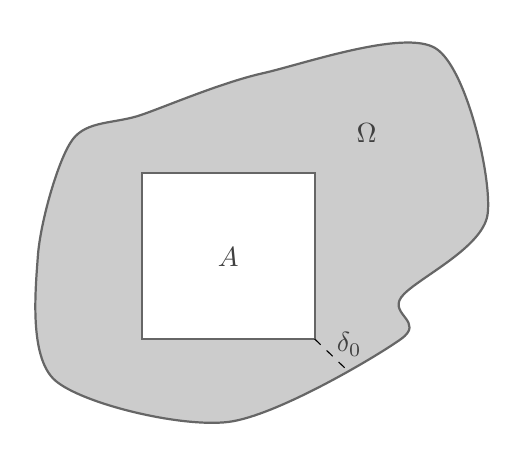
\begin{tikzpicture}
			 \begin{axis}[axis x line=none, axis y line=none]
				\addplot[mark=none, black!60, smooth cycle, thick, fill=gray!40] coordinates {(1,1) (2,0.5) (3,1.5) (3,2) (3.5,3) (3.2, 5) (2.2, 4.7) (1.5, 4.2) (1.1, 3.9) (0.9, 2.5)};
				\node[black!75] at (axis cs:2.8,3.75) [anchor=south] {$\Omega$};
				\addplot[mark=none, black!60, thick, fill=white!30] coordinates {(2.5,1.5) (2.5,3.5) (1.5,3.5) (1.5,1.5) (2.5,1.5)};
				\node[black!75] at (axis cs:2,2.25) [anchor=south] {$A$};
				\addplot[dashed] coordinates {(2.5,1.5) (2.7,1.1)};
				\node[black!75] at (axis cs:2.7,1.175) [anchor=south] {$\delta_{0}$};
			 \end{axis}
			\end{tikzpicture}
		\end{figure}
			
		Da $\supp(\phi_{\delta}) \subset B(0, \delta)$ nach \hyperref[bem:8.7ii]{8.7 ii)}
		\[ \Rightarrow \supp(g \ast \phi_{\delta} ) \subset A + B\left(0, \frac{\delta_{0}}{2}\right) \subset \Omega \text{ für } \delta < \frac{\delta_{0}}{2} \]
		(mit $A + B \coloneqq \{ x + y : x \in A, y \in B\}$), denn $g \ast \phi_{\delta}(u) = \int \phi_{\delta}(u - v) g(v) dv \neq 0$ nur wenn $v \in A$ und $\| u - v \| < \delta$. \\
		Also $g \ast \phi_{\delta} \in C_{c}(\Omega)$. Zu zeigen: $g \ast \phi_{\delta} \in C^{\infty}(\Omega)$
		\[ D_{u}^{\alpha}(\phi_{\delta} \ast g)(u) = \int_{A} \left[ D_{u}^{\alpha} \phi_{\delta}(u - v) \right] \underbrace{g(v)}_{\text{beschränkt}} gv \]
		d.h. $\phi_{\delta} \ast g \in C	^{\infty}$; in einfachen Worten bedeutet das, dass $C_{\delta} \ast g$ alle guten Eigenschaften von $\phi$ $"$erbt$"$, auch wenn $g$ $"$schlecht$"$ ist. \\
		\[ \| f - \phi_{\delta} \ast g \|_{L^{p}} \leq \underbrace{\| f - g \|}_{\leq \epsilon} + \underbrace{\| g - \phi_{\delta} \ast g \|_{L^{p}}}_{\leq \epsilon} \text{ für } \epsilon \text{ klein genug nach } \hyperref[satz:8.8]{8.8} \]
	\end{beweis}
\end{kor}


\begin{bemerkung*}
	Es gilt:
	\begin{itemize}
		\item $\supp(f) \subset A, \supp(g) \subset B \quad \Rightarrow  \quad \supp(f + g) \subset A + B $
		\item $f \ast g = g \ast f$
	\end{itemize}	
\end{bemerkung*}


\begin{kor} \label{kor:8.10}
	Sei $\Omega \subseteq \MdR^{d}$ offen. Sei $f \in L^{p}(\Omega), p \in [1, \infty)$ mit $\int f(u) g(u) du = 0$ für alle $g \in C_{c}^{\infty}(\Omega)$. Dann ist $f = 0$.
	\begin{beweis}
		Zu $f \in L^{p}$ gibt es ein $g \in L^{p'}, \frac{1}{p} + \frac{1}{p'} = 1$ mit 
		\[ \| f \|_{L^{p}} = \int f(u) g(u) du, \quad \| g \|_{L^{p'}} = 1 \]
		Wähle $g(u) = |f(u)|^{p - 1} \left( sign(f(u)) \right) \cdot \| f \|_{L^{p}}^{\frac{1}{p} - 1}$. Dann ist
		\begin{align*}
			\| f \|_{L^{p}} & = \left( \int |f(u)|^{p} du \right)^{\frac{1}{p}} = \| f \|_{L^{p}}^{\frac{1}{p} - 1} \int |f(u)|^{p} du \\
			& = \int f(u) \underbrace{\frac{sign(f(u)) |f(u)|^{p - 1}}{\| f \|^{1 - \frac{1}{p}}}}_{=: g(u)} du \\
			& = \int f(u) g(u) du
		\end{align*}
		$\| g \|_{L^{p'}} = 1$ mit $\frac{1}{p} + \frac{1}{p'} = 1$. (sieh auch \hyperref[satz:8.1]{Beweis 8.1}) 
		\[ \| f \|_{L^{p}} = \int f(u) g(u) du = \int f(u) [g(u) - \phi(u)] du \text{ für alle } \phi \in C_{c}^{\infty}(\Omega), \quad \text{ denn } \int f(u) \phi(u) du = 0 \]
		Wähle nach \hyperref[kor:8.9]{8.9} ein $\phi \in C_{c}^{\infty}(\Omega)$ mit $\| g - \phi \|_{L^{p'}(\Omega)} < \frac{1}{2}$ \\ \\
		Also $\| f \|_{L^{p}} \underset{\text{Hölder}}{\leq} \| f \|_{L^{p}} \| f - \phi \|_{L^{p'}} < \frac{1}{2} \| f \|_{L^{p}}$, was einen Widerspruch zu $f \neq 0$ darstellt, demnach gilt $\| f \|_{L^{p}} = 0, f = 0$.
	\end{beweis}
\end{kor}



\newpage	